\documentclass[a4paper]{article}
\usepackage{fullpage}
\usepackage{amsmath}
\usepackage{amssymb}
\usepackage{breqn}
\usepackage{sectsty}
\usepackage{graphicx}
\usepackage{svg}
\usepackage{xcolor}
\usepackage{esint}
\usepackage{pdfpages}
\usepackage{fancyhdr}
\usepackage{chngcntr}
\usepackage{pagecolor}
\usepackage{caption}
\usepackage{subcaption}
\usepackage{physics}
\usepackage{float}
\counterwithin*{equation}{section}
\counterwithin*{equation}{subsection}
\renewcommand{\thesubsection}{\thesection.\alph{subsection}}
\renewcommand{\thesubsubsection}{\Roman{subsubsection}}
\newcommand{\horln}{\vspace{-6mm}\begin{flushleft}\mbox{}\hrulefill\mbox{}
	\end{flushleft}\vspace{-6mm}}
\newcommand\eq{\addtocounter{equation}{1}\tag{\theequation}}
\sectionfont{\huge}
\subsubsectionfont{\small}
\setlength{\parindent}{0cm}
\usepackage[citestyle=ieee]{biblatex}
\title{PHYS4123 GR Assignment 1}
\author{SID: 480344342}
\begin{document}
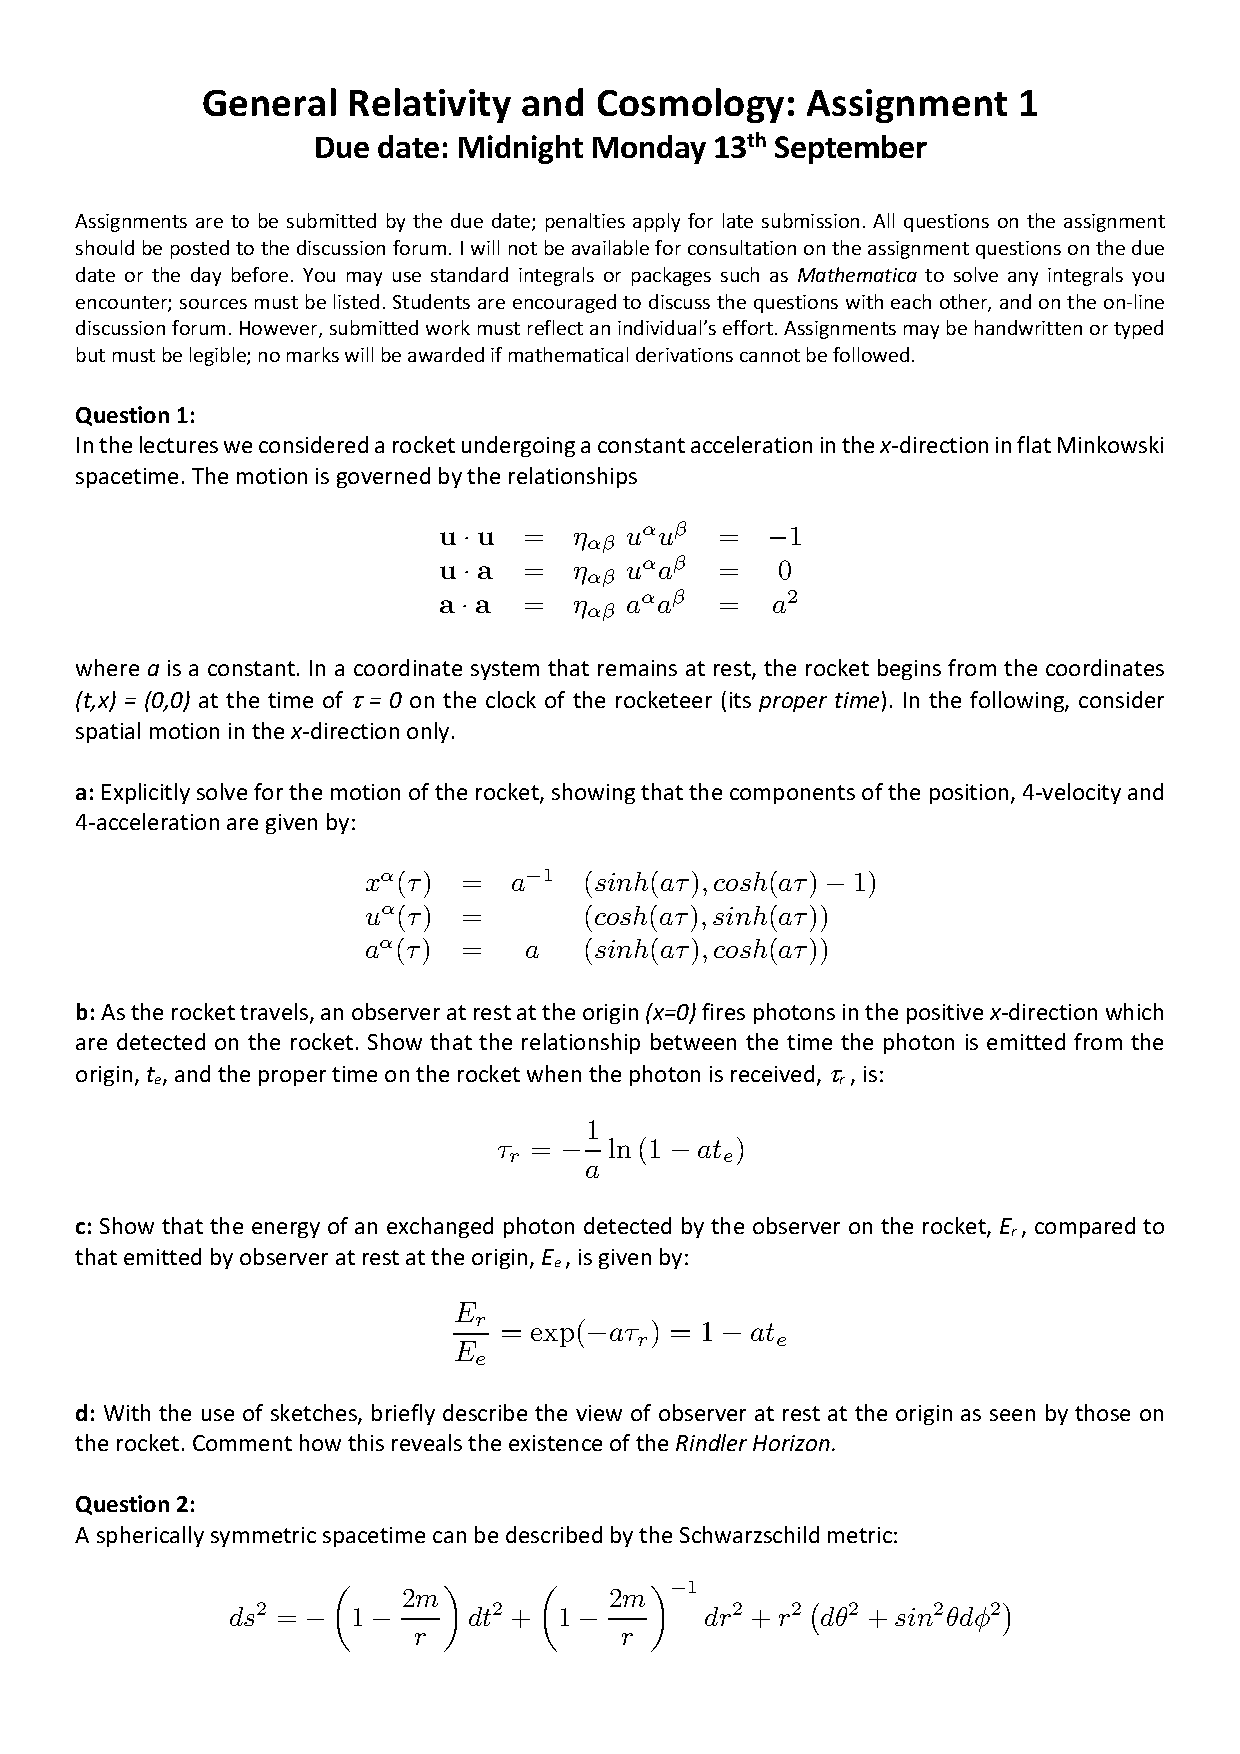
\includepdf[pages=-]{Figures/Questions}
\maketitle
\horln

\setcounter{page}{1}

%  *  ██████   ██
%  * ██    ██ ███
%  * ██    ██  ██
%  * ██ ▄▄ ██  ██
%  *  ██████   ██
%  *     ▀▀

\section{}
\subsection{}
\begin{align*}-1 &= \eta_{\alpha \beta} u^\alpha u^\beta\\
0 &= \eta_{\alpha \beta} u^\alpha a^\beta \\
a^2 &= \eta_{\alpha \beta} a^\alpha a^\beta
\end{align*}
Assuming spatial motion only occurs in $x^1$ gives:
\begin{align*}
-1 &= -u^0u^0 + u^1u^1\\
0 &= -u_0a_0 + u_1 a_1\\
a^2 &= -a^0a^0 + a^1a^1
\end{align*}
Then:
\begin{align*}
u^0u^0 &= u^1u^1 + 1 \eq \label{eq:1}\\
a_0 &= \frac{u_1}{u_0} a_1 \eq \label{eq:2}\\
a^1a^1 &= a^0a^0 + a^2 \eq \label{eq:3}
\end{align*}

Substituting \eqref{eq:2} into \eqref{eq:3}:
\begin{align*}
a^1a^1 &= a^2 \frac{1}{1-u^1u^1/u^0u^0}\\
a^0a^0 &= a^2 \frac{1}{u^0u^0/u^1u^1 - 1}
\end{align*}

Then using \eqref{eq:1}:
\begin{align*}
a^1a^1 &= a^2 (1 + u^1 u^1) = \left(\frac{du^1}{d\tau}\right)^2\\
a^0a^0 &=  a^2 (u^0 u^0 - 1) =  \left(\frac{du^0}{d\tau}\right)^2
\end{align*}

Integrating:
\begin{align*}
\tau &= \pm \int \frac{1}{\abs{a}\sqrt{1 + u^1 u^1}} du^1 = \pm \frac{1}{\abs{a}}\sinh^{-1}(u^1) + A\\
\tau &= \pm \int \frac{1}{\abs{a}\sqrt{u^0 u^0 - 1}} du^1 = \pm \frac{1}{\abs{a}}\cosh^{-1}(u^0) + B
\end{align*}
Assuming $u^0 > 0$. Since the rocket begins at rest, $(u^0, u^1) = (1, 0)$ at $\tau = 0$ and$C = 0$ and $B = 0$. Also, letting $\mp \abs{a} = a$ (such that the sign of $a$ is the direction of $a^1$):
\begin{align*}
(u^0, u^1) &= (\cosh(a \tau), \sinh(a\tau))
\end{align*}
Differentiating gives:
\begin{align*}
	(a^0, a^1) &= a(\sinh(a \tau), \cosh(a\tau))
\end{align*}
Whereas integrating gives:
\begin{align*}
	(x^0, x^1) &= \frac{1}{a}(\sinh(a \tau) + C, \cosh(a\tau) + D)
\end{align*}
Where the initial conditions $(x^0, x^1) = (0, 0)$ at $\tau = 0$ constrain $C = 0$ and $D = -1$.



\subsection{}
As shown in figure~\ref{fig:1}, a photon launched at $t_e$ by a stationary observer will intersect with the world line of the rocket (as long as $t_e$ is less than some critical value). 
The photon's world line is a straight line with gradient $1$ (a speed of $c$) intersecting $x=0$ at $t_e$.
The rocket's world line is the curve $(x, t) = x^\alpha(\tau)$, derived in part $a$.
The intersection of these two world lines occurs when:
\begin{align*}
	x &= t - t_e\\
	\implies \frac{1}{a}\cosh(a\tau_r) - \frac{1}{a} &= \frac{1}{a} \sinh(a\tau_r) - t_e\\
	\implies 1-at_e &= \cosh(a\tau_r) - \sinh(a\tau_r) \\
	&= e^{-a \tau_r}\\
	\implies -a \tau_r &= \ln(1-at_e)\\
	\implies \tau_r &= -\frac{1}{a} \ln(1-at_e)
\end{align*}



\subsection{}

The relativistic Doppler shift with an angle of $0$ between a photon and a target is:
$$E_r = E_e\sqrt{\frac{1 - v}{{1 + v}}},$$
where $E_e$ is the energy of the photon in the rest frame of the source moving at $-v$ relative to the rocket, which receives a photon of energy $E_r$.
The rocket's velocity at the time of receiving the photon is:
$$v(\tau_r) = \frac{dx}{dt} = \frac{dx}{d\tau} \cdot \frac{d\tau}{dt} = \frac{u^x(\tau_r)}{u^t(\tau_r)} = \tanh(a\tau_r)$$
Therefore:
\begin{align*}
	\frac{E_r}{E_e} &= \sqrt{\frac{1 - \tanh(a\tau_r)}{{1 + \tanh(a\tau_r)}}}\\
	&=  \sqrt{\frac{1- \frac{\exp({2a\tau_r}) - 1}{\exp({2a\tau_r}) + 1}}{1 + \frac{\exp({2a\tau_r}) - 1}{\exp({2a\tau_r}) + 1}}}\\
	&=  \sqrt{\frac{\exp({2a\tau_r}) + 1 - \exp({2a\tau_r}) + 1}{\exp({2a\tau_r}) + 1 + \exp({2a\tau_r}) - 1}}\\
	%&=  \sqrt{\frac{2}{2\exp({2a\tau_r})}}\\
	&=  e^{-a\tau_r}.
\end{align*}
From the previous part, this also means $ \frac{E_r}{E_e} = 1 - a t_e$.


\begin{figure}[H]
	{ \centering
		 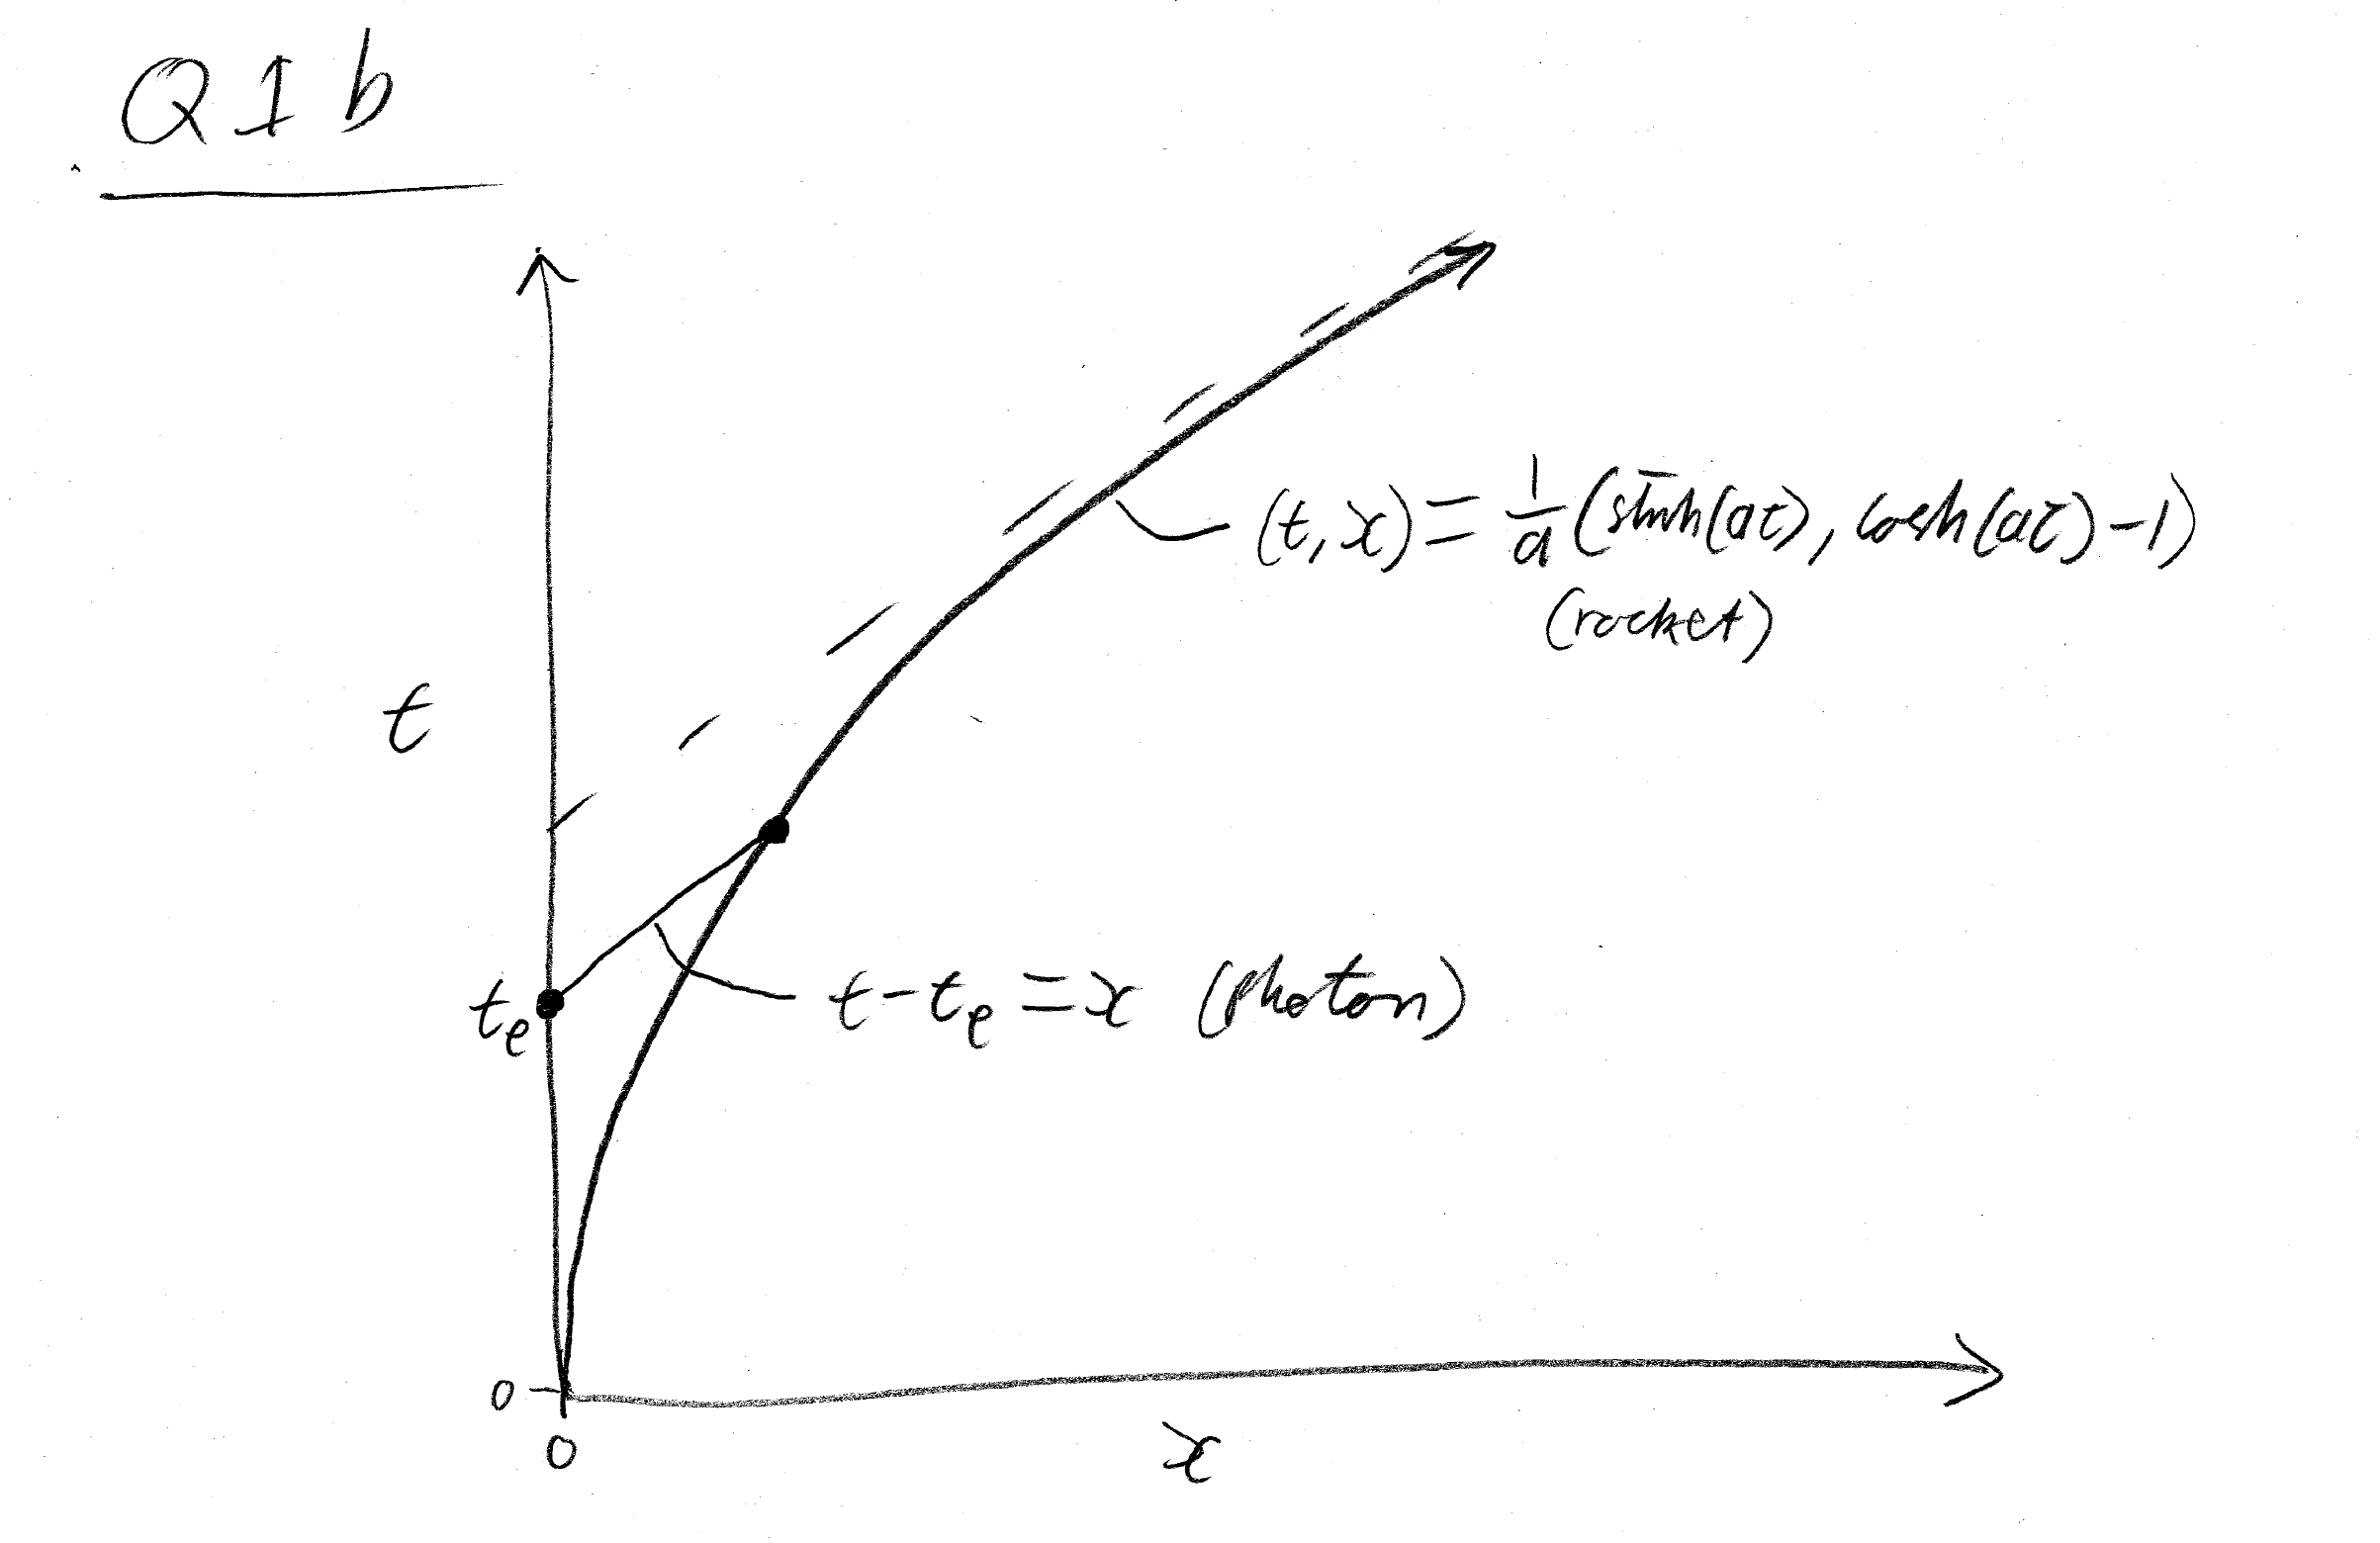
\includegraphics[width=\textwidth]{Figures/1b}
		 \caption{\textbf{A photon launched at an accelerating rocket.} The time at which the rocket receives the photon can be calculated from the intersection of their world lines.}
	 \label{fig:1}}
	 {\centering
		 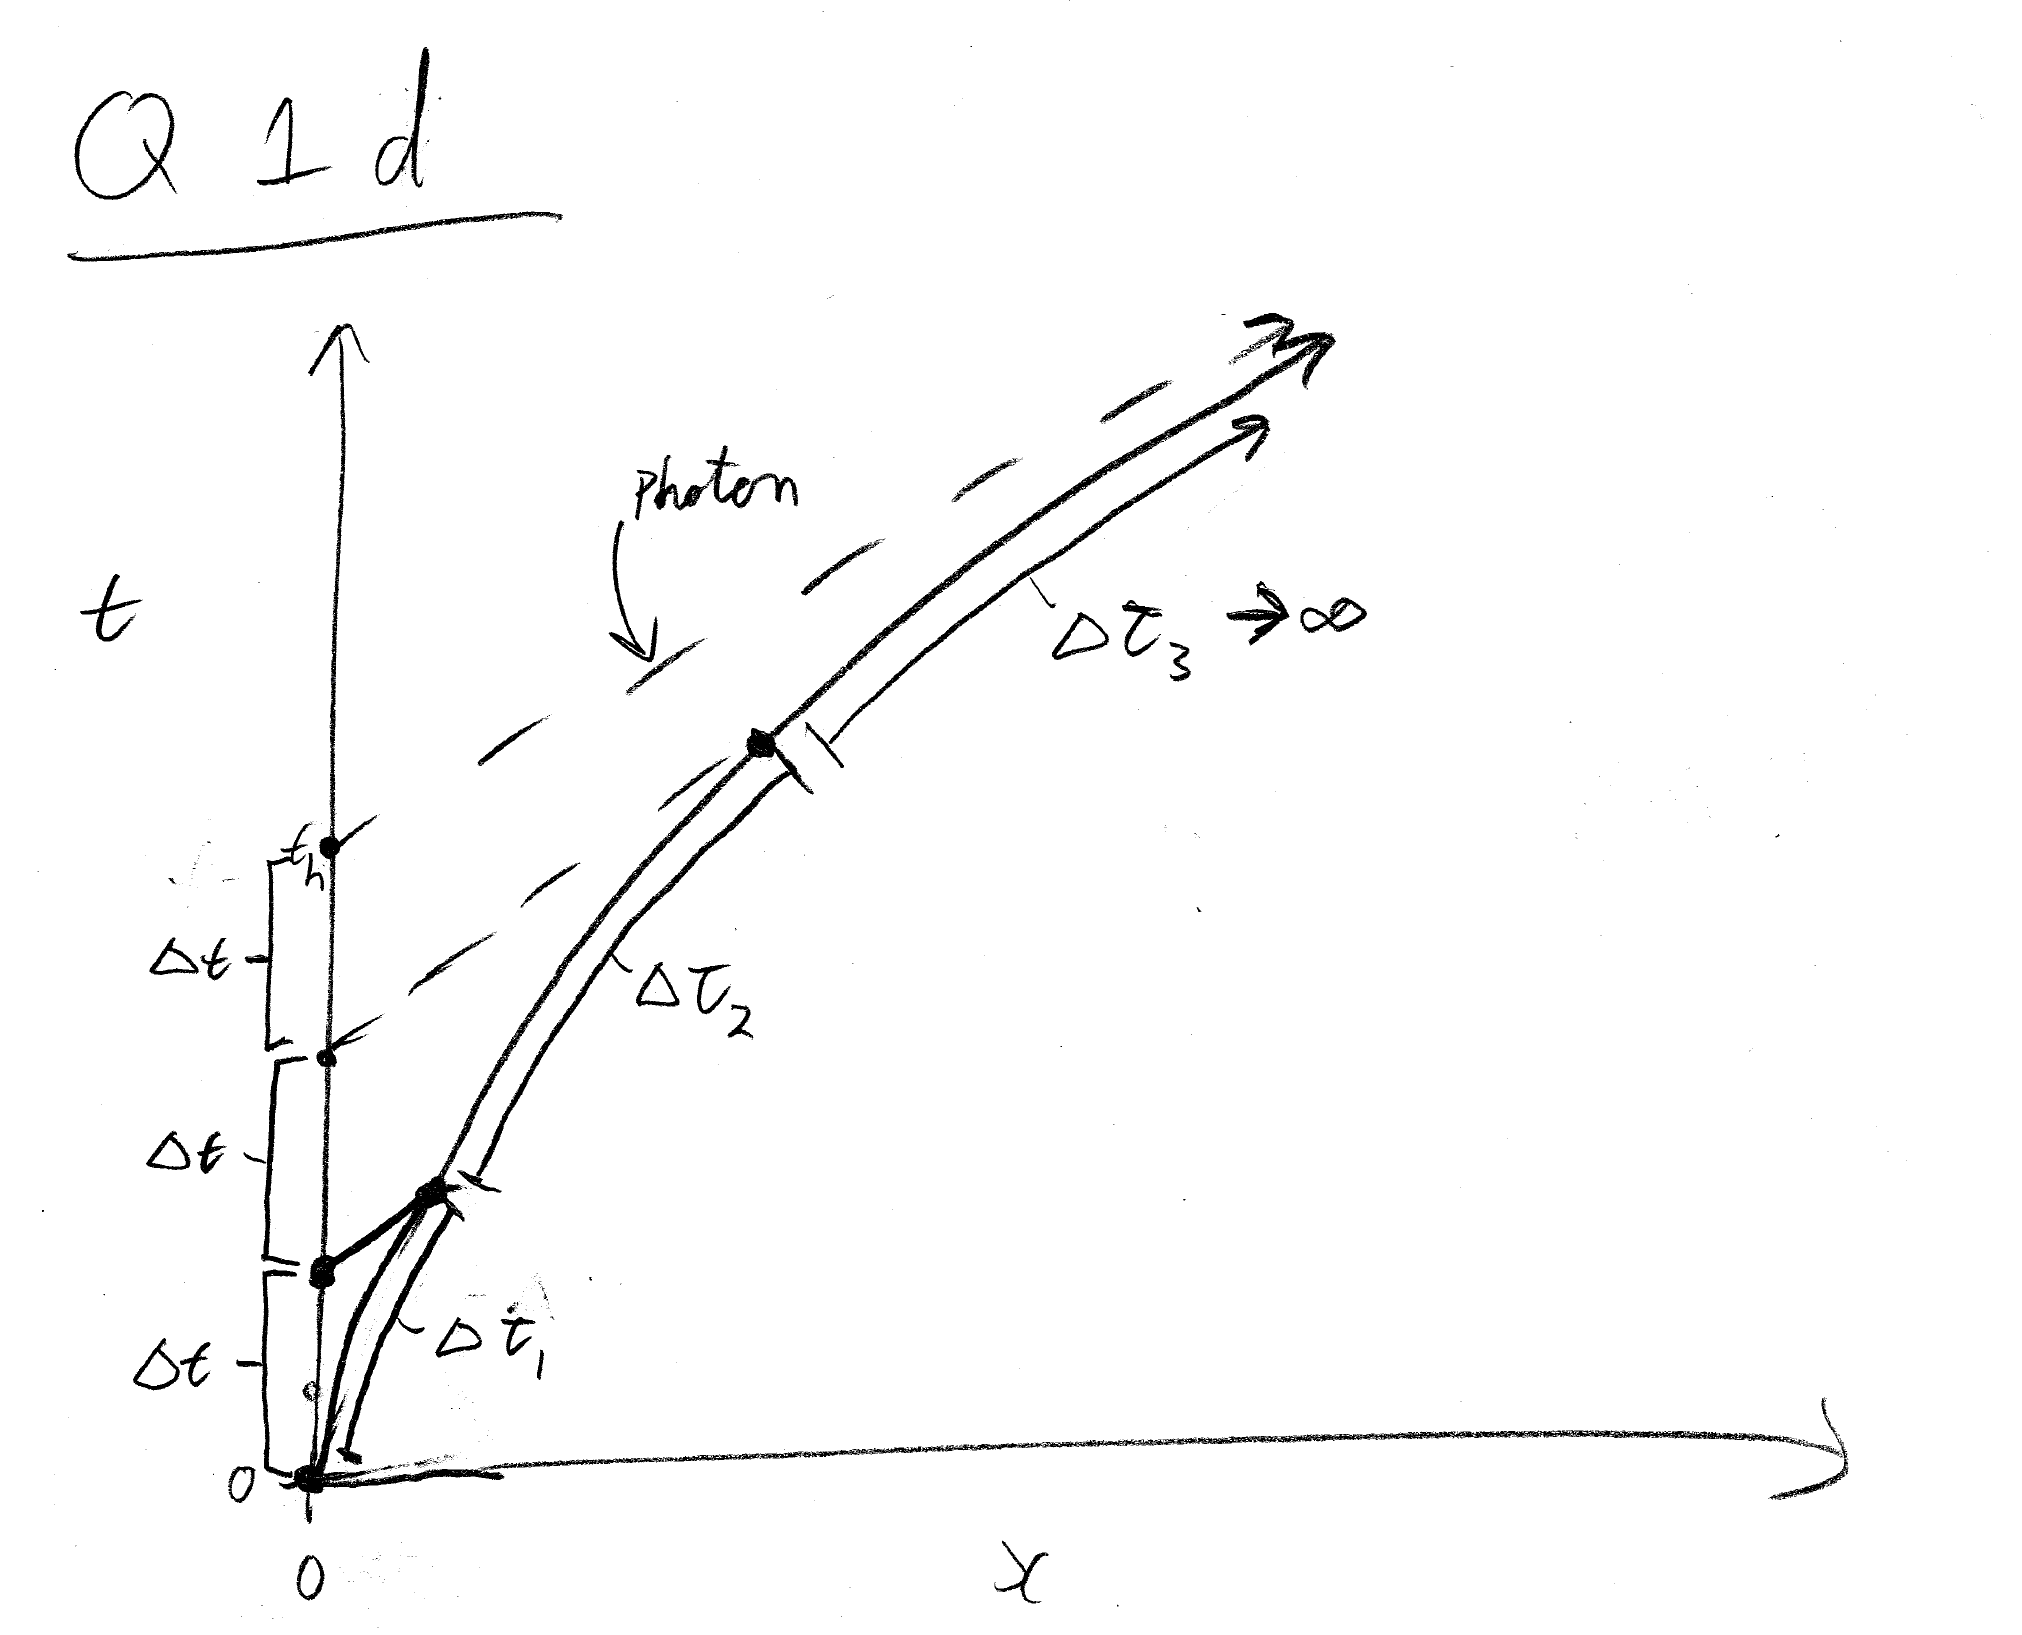
\includegraphics[width=0.85\textwidth]{Figures/1d}
		 \caption{\textbf{Successive photons launched at an accelerating rocket}. The length of intervals between received photons along the rocket's world line increases to infinity for photons launched at equally spaced intervals by a  non-accelerating observer. }
	 \label{fig:2}}
 \end{figure}


\subsection{}
The velocity of the rocket, measured by the stationary observer, asymptotically approaches the speed of light, as indicated by the equations derived in part $a$. 
This means the gradient of the rocket's world line approaches unity, shown in figure~\ref{fig:1}. 
If the rocket observes the stationary observer, what it sees will slow down increasingly as it accelerates.
For example, figure~\ref{fig:2} shows the world-lines of a scenario in which the stationary observer sends a photon to the moving rocket at regular intervals of $\Delta t$ (in the stationary observers own time).
While they have a small acceleration, the proper time of the moving rocket at which it receives the photon (related to the length of its world line) will be slightly larger than the time at which the stationary observer emits the photon. This discrepancy between $\Delta \tau_1$ incorporates both the travel time of the photon and the acceleration of the rocket, since and this proper time is also larger than the time at which the photon arrives at the rocket.
At the second increment, $2\Delta t$, another photon is emitted by the stationary observer.
The proper time at which it arrives at the rocket is again greater than the coordinate time, and moreso. 
Hence the time between equally spaced events in the stationary observers frame is increased when viewed by the rocket, so the rocket's view of the origin is slowed-down as it accelerates.
Finally, the third photon emitted by the stationary observer has a world-line that is asymptotic to world-line of the rocket. 
The rocket never receives this photon; the rockets view of the stationary observer becomes 'frozen' as it approaches this critical time, $t_h$ (the third interval of proper time, $\Delta \tau_3$, is infinite, assuming the rocket never ceases accelerating).
This represents the Rindler horizon; no signals emitted by the observer later $t_h$ can be received by the rocket.
The Rindler horizon is clear from the equation in part $c$, which shows the proper time at which emitted photons are received asymptotes to $\infty$ as $t_e \to \frac{1}{a} = t_h$.
There is also a point behind the origin (the intersection of the light line passing through the original at $t_h$) that the rocket cannot view past, although the rocket will see points closer than this spatial horizon (such as the origin) approach it asymptotically.
The image of the origin will also appear red-shifted as the rocket gains velocity, and fainter as it gains distance.




%  *  ██████  ██████▄
%  * ██    ██      ██
%  * ██    ██ ▄█████▀
%  * ██ ▄▄ ██ ██
%  *  ██████  ███████
%  *     ▀▀

\section{}
\subsection{}
% Since the proper time is:
% \begin{align*}
% 	\tau = \int_0^1 -d\sigma ds,
% \end{align*}
% for some parameterisation by $\sigma$ of a path is spacetime, 
The Lagrangian equivalent $K$ for the Schwarzschild metric is:
\begin{align*}
	K &= g_{\alpha \beta} \frac{dx^\alpha}{d\tau} \frac{dx^\beta}{d\tau}\\
	&=	-\left( 1- \frac{2m}{r}\right) \left( \frac{dt}{d\tau} \right)^2 + \left( 1- \frac{2m}{r}\right)^{-1} \left( \frac{dr}{d\tau} \right)^2    + r^2 \left( \frac{d\theta}{d\tau} \right)^2  + r^2 \sin^2(\theta) \left( \frac{d\phi}{d\tau} \right)^2  . 
\end{align*}
Then:
\begin{align*}
\frac{\partial K}{\partial \left(dx^\alpha / d\tau \right)} &= 2\left[-\left( 1- \frac{2m}{r}\right) \frac{dt}{d\tau} , \left( 1- \frac{2m}{r}\right)^{-1} \frac{dr}{d\tau} , r^2 \frac{d\theta}{d\tau} , r^2 \sin^2(\theta) \frac{d\phi}{d\tau} \right], \\
%\implies \frac{d}{d\tau} \frac{\partial K}{\partial \left(dx^\alpha / d\tau \right)}  &= 2 \left[-\left( 1- \frac{2m}{r}\right) \frac{d^2t}{d\tau^2} , \left( 1- \frac{2m}{r}\right)^{-1} \frac{d^2r}{d\tau^2} , r^2 \frac{d^2\theta}{d\tau^2} , r^2 \sin^2(\theta) \frac{d^2\phi}{d\tau^2} \right] \\
\intertext{and:}
\frac{\partial K}{\partial x^\alpha} &= 2\left[0, \frac{1}{2}\frac{\partial K}{\partial r}, r^2 \sin(\theta)\cos(\theta) \left( \frac{d\phi}{d\tau} \right)^2, 0 \right],
\end{align*}
where:
\begin{align*}
	\frac{1}{2}\frac{\partial K}{\partial r} &= -\frac{m}{r^2} \left(\frac{dt}{d\tau} \right)^2 - \frac{m}{(r-2m)^2}  \left(\frac{dr}{d\tau} \right)^2 + r  \left(\frac{d\theta}{d\tau} \right)^2  + r\sin^2(\theta)  \left(\frac{d\phi}{d\tau} \right)^2.
\end{align*}
Using the Euler-Lagrange equation:
\begin{align*}
\frac{d}{d\tau} \frac{\partial K}{\partial(dx^\alpha / d\tau)}  = \frac{\partial K}{\partial x^\alpha},
\end{align*}
gives:
\begin{align*}
	\frac{d}{d\tau} \left[ \left(1-\frac{2m}{r}\right) \frac{dt}{d\tau} \right] &= 0\\
	\frac{d}{d\tau} \left[ \left( 1- \frac{2m}{r}\right)^{-1} \frac{dr}{d\tau} \right] &=  -\frac{m}{r^2} \left(\frac{dt}{d\tau} \right)^2 - \frac{m}{(r-2m)^2}  \left(\frac{dr}{d\tau} \right)^2 + r  \left(\frac{d\theta}{d\tau} \right)^2  + r\sin^2(\theta)  \left(\frac{d\phi}{d\tau} \right)^2\\
	\frac{d}{d\tau} \left[ r^2 \frac{d\theta}{d\tau}  \right]  &= r^2 \sin(\theta)\cos(\theta) \left( \frac{d\phi}{d\tau} \right)^2 \\
	\frac{d}{d\tau} \left[r^2 sin^2(\theta) \frac{d\phi}{d\tau} \right] &= 0
\end{align*}



\subsection{}
Expanding and rearranging the equations of motion above:
\begin{align*}
	0 &= \left(1-\frac{2m}{r}\right) \frac{d^2 t}{d\tau^2}  + \frac{dt}{d\tau} \frac{2m}{r^2} \frac{dr}{d\tau} \\
	\frac{d^2r}{d\tau^2} \frac{r}{r-2m} - \left(\frac{dr}{dt}\right)^2 \frac{2m}{(r-2m)^2}&=   -\frac{m}{r^2} \left(\frac{dt}{d\tau} \right)^2 - \frac{m}{(r-2m)^2}  \left(\frac{dr}{d\tau} \right)^2 + r  \left(\frac{d\theta}{d\tau} \right)^2  + r\sin^2(\theta)  \left(\frac{d\phi}{d\tau} \right)^2 \\
	r^2 \frac{d^2\theta}{d\tau^2} + 2r \frac{dr}{d\tau} \frac{d\theta}{d\tau}  &= r^2 \sin(\theta)\cos(\theta) \left( \frac{d\phi}{d\tau} \right)^2 \\
	0 &= r^2 \sin^2(\theta) \frac{d^2\phi}{d\tau^2} + 2r \sin^2(\theta) \frac{d\phi}{d\tau}\frac{dr}{d\tau} + 2r^2 \cos(\theta) \sin(\theta) \frac{d\theta}{d\tau} \frac{d\phi}{d\tau}
\end{align*}
Then:
\begin{align*}
	\frac{d^2 t}{d\tau^2} &= - \frac{2m}{r^2} \left(1-\frac{2m}{r}\right)^{-1} \frac{dt}{d\tau}  \frac{dr}{d\tau}\\
	\frac{d^2r}{d\tau^2} &=   -\frac{m}{r^2} \left(1-\frac{2m}{r}\right) \left(\frac{dt}{d\tau} \right)^2 + \frac{m}{r^2\left(1-\frac{2m}{r}\right)}  \left(\frac{dr}{d\tau} \right)^2 + (r - 2m)  \left(\frac{d\theta}{d\tau} \right)^2  + (r - 2m)\sin^2(\theta)  \left(\frac{d\phi}{d\tau} \right)^2\\
	\frac{d^2\theta}{d\tau^2}  &= \sin(\theta)\cos(\theta) \left( \frac{d\phi}{d\tau} \right)^2 - \frac{2}{r} \frac{dr}{d\tau} \frac{d\theta}{d\tau} \\
	 \frac{d^2\phi}{d\tau^2} &= - \frac{2}{r}  \frac{d\phi}{d\tau}\frac{dr}{d\tau} - 2 \frac{\cos(\theta)}{ \sin(\theta)} \frac{d\theta}{d\tau} \frac{d\phi}{d\tau}
\end{align*}
The general geodesic equation is:
\begin{align*}
\frac{d^2 x^\alpha}{d\tau^2} &= -\Gamma^\alpha_{\beta \gamma} \frac{dx^\beta}{d\tau}\frac{dx^\gamma}{d\tau}
\end{align*}
Comparing the rearranged equations of motion to the general geodesic equation gives:
\begin{align*}\
	\begin{split}
	\Gamma^t_{r t} &=  \Gamma^t_{t r} = \left(1-\frac{2m}{r}\right)^{-1} \frac{m}{r^2}\\
	\Gamma^r_{tt} &=  \left( 1 - \frac{2m}{r} \right) \frac{m}{r^2}\\
\Gamma^r_{rr} &=   -\frac{m}{r^2} \left(1-\frac{2m}{r}\right)^{-1} \\
\Gamma^r_{\theta \theta} &=  -\left( r - 2m \right)
	\end{split}
	\begin{split}
\Gamma^r_{\phi \phi} &=  -\left( r - 2m \right) \sin^2(\theta)\\
\Gamma^\theta _{\theta r} &= \Gamma^\theta _{r \theta} = \frac{1}{r}\\
\Gamma^\theta _{\phi \phi} &=  -\sin(\theta) \cos(\theta)\\
\Gamma^\phi_{\phi r} &= \Gamma^\phi_{r \phi} =  \frac{1}{r}\\
\Gamma^\phi_{\theta \phi} &= \Gamma^\phi_{\phi \theta} = \frac{ \cos(\theta)}{\sin(\theta)}
	\end{split}
\end{align*}
Note that for symbols with two unique lower indices the coefficients of the equations of motion are halved (one half to each ordering of the indices/derivatives, to ensure the symbols are symmetric).

\subsection{}

The metric is:
\begin{align*}
	g_{\alpha\beta} &= \begin{bmatrix} -\left(1-\frac{2m}{r}\right) & 0 & 0 & 0 \\
		0 & \left( 1 - \frac{2m}{r} \right)^{-1} & 0 & 0\\
		0 & 0 & r^2 & 0 \\
		0 & 0 & 0 & r^2 \sin^2(\theta)
	\end{bmatrix}\\
\end{align*}

Since the metric is diagonal ($g^{\alpha \delta} = 0$ when $\alpha \ne \delta$), the relationship between the metric and the Christoffel symbols can be simplified to:
$$\Gamma^\alpha_{\beta \gamma} = \frac{1}{2} g^{\alpha \alpha}(g_{\alpha \beta , \gamma} + g_{\alpha \gamma , \beta} - g_{\beta \gamma , \alpha}), $$
since all other terms are zero. 
Also, the lower indices can be interchanged since Christoffel symbols are symmetric.


\subsubsection{$\boldsymbol{\Gamma^t_{\beta \gamma}}$}
Then for $\alpha = t$, $g_{\beta\gamma,t} = 0$ and:
\begin{align*}
	\Gamma^t_{\beta \gamma} &= \frac{1}{2} g^{tt}(g_{t\beta , \gamma} + g_{t \gamma , \beta})\\
	&= \frac{1}{2} g^{tt} \begin{bmatrix} 0 & -\frac{2m}{r^2} & 0 & 0 \\
		-\frac{2m}{r^2} & 0 & 0 & 0\\
		0 & 0 & 0 & 0 \\
		0 & 0 & 0 & 0
\end{bmatrix}\\
\implies \Gamma^t_{r t} &=  \Gamma^t_{t r} = \left(1-\frac{2m}{r}\right)^{-1} \frac{m}{r^2}
\end{align*}
where all other symbols are 0.

\subsubsection{$\boldsymbol{\Gamma^r_{\beta \gamma}}$}
If $\alpha = r$:
\begin{align*}
	g_{\beta\gamma,r} &= \begin{bmatrix} -\frac{2m}{r^2} & 0  & 0 & 0 \\
				0 & -\frac{2m}{(r-2m)^2} & 0 & 0\\
				0 & 0 & 2r & 0  \\
				0 & 0 & 0 & 2r\sin^2(\theta)
			\end{bmatrix}
\end{align*}
And:
\begin{align*}
	g_{r\beta , \gamma} + g_{r \gamma , \beta} &= \begin{bmatrix} 0 & 0 & 0 & 0 \\
		0 & -\frac{4m}{(r-2m)^2} & 0 & 0\\
		0 & 0 & 0 & 0 \\
		0 & 0 & 0 & 0
\end{bmatrix}\\
\implies 	g_{r\beta , \gamma} + g_{r \gamma , \beta} - g_{\beta\gamma,r} &= \begin{bmatrix} \frac{2m}{r^2} & 0 & 0 & 0 \\
	0 & -\frac{2m}{(r-2m)^2} & 0 & 0\\
	0 & 0 & -2r & 0  \\
	0 & 0 & 0 & -2r\sin^2(\theta)
\end{bmatrix}\\
\implies \Gamma^r_{tt} &=  \left( 1 - \frac{2m}{r} \right) \frac{m}{r^2}\\
\Gamma^r_{rr} &=  -\left( 1 - \frac{2m}{r} \right) \frac{m}{(r-2m)^2} =  -\frac{m}{r^2} \left(1-\frac{2m}{r}\right)^{-1} \\
\Gamma^r_{\theta \theta} &=  -\left( 1 - \frac{2m}{r} \right) r =  -\left( r - 2m \right) \\
\Gamma^r_{\phi \phi} &=  -\left( 1 - \frac{2m}{r} \right) -2r\sin^2(\theta) =  -\left( r - 2m \right) \sin^2(\theta)
\end{align*}


\subsubsection{$\boldsymbol{\Gamma^\theta_{\beta \gamma}}$}
If $\alpha = \theta$:
\begin{align*}
	g_{\beta\gamma,\theta} &= \begin{bmatrix} 0 & 0  & 0 & 0 \\
				0 &0 & 0 & 0\\
				0 & 0 & 0 & 0  \\
				0 & 0 & 0 & 2r^2 \sin(\theta) \cos(\theta)
			\end{bmatrix}
\end{align*}
And:
\begin{align*}
	g_{\theta\beta , \gamma} + g_{\theta \gamma , \beta} &= \begin{bmatrix} 0 & 0 & 0 & 0 \\
		0 & 0 & 2r & 0\\
		0 & 2r & 0 & 0 \\
		0 & 0 & 0 & 0
\end{bmatrix}\\
\implies 	g_{\theta\beta , \gamma} + g_{\theta \gamma , \beta} - g_{\beta\gamma,\theta} &= \begin{bmatrix} 0 & 0 & 0 & 0 \\
	0 & 0 & 2r & 0\\
	0 & 2r & 0 & 0 \\
	0 & 0 & 0 & -2r^2 \sin(\theta) \cos(\theta)
\end{bmatrix}\\
\implies \Gamma^\theta _{\theta r} &= \Gamma^\theta _{r \theta} = \frac{1}{2} r^{-2} 2r = \frac{1}{r}\\
\Gamma^\theta _{\phi \phi} &= -\frac{1}{2} r^{-2} 2r^2\sin(\theta)\cos(\theta) = -\sin(\theta) \cos(\theta)
\end{align*}

\subsubsection{$\boldsymbol{\Gamma^\theta_{\beta \gamma}}$}
Finally, if $\alpha = \phi$ then $g_{\beta\gamma,\phi} = 0$ and:
\begin{align*}
	g_{\phi\beta , \gamma} + g_{\phi \gamma , \beta} &= \begin{bmatrix} 0 & 0 & 0 & 0 \\
		0 & 0 & 0 & 2r\sin^2(\theta)\\
		0 & 0 & 0 & 2r^2 \sin(\theta)\cos(\theta) \\
		0 & 2r\sin^2(\theta) & 2r^2 \sin(\theta)\cos(\theta) & 0
\end{bmatrix}\\
\implies \Gamma^\phi_{\phi r} &= \Gamma^\phi_{r \phi} = \frac{1}{2} r^{-2}\sin^{-2}(\theta) \cdot 2r \sin^2(\theta) =  \frac{1}{r}\\
\Gamma^\phi_{\theta \phi} &= \Gamma^\phi_{\phi \theta} = \frac{1}{2}r^{-2}\sin^{-2}(\theta) \cdot 2r^2\sin(\theta)\cos(\theta) = \frac{ \cos(\theta)}{\sin(\theta)}
\end{align*}
% Regrouping:
% \begin{align*}
% 	\Gamma^\alpha_{\beta \gamma} &= \frac{1}{2} g^{\alpha } (g_{\beta , \gamma} + g_{\gamma , \beta}) - \frac{1}{2}g^{\alpha \alpha}g_{\beta \gamma , \alpha}
% \end{align*}
% where $g^\alpha$ sums over the diagonal of $g^{\alpha \alpha}$ (as for $g_\gamma$ and $g_\beta$).


% Then:
% \begin{align*}
% 	 g_{\beta, \gamma} &= \begin{bmatrix} 0 & -\frac{2m}{r^2}  & 0 & 0 \\
% 			0 &\frac{-2m}{(r-2m)^2} & 0 & 0\\
% 			0 & 2r & 0 & 0 \\
% 			0 & 2r\sin(\theta) & 2r^2 \sin(\theta) \cos(\theta) & 0
% 		\end{bmatrix}\\
% % g_{\beta \gamma, \alpha} &= \begin{bmatrix} -\left(1-\frac{2m}{r}\right) & 0 & 0 & 0 \\
% % 			0 & \left( 1 - \frac{2m}{r} \right)^{-1} & 0 & 0\\
% % 			0 & 0 & r^2 & 0 \\
% % 			0 & 0 & 0 & r^2 \sin^2(\theta)
% % \end{bmatrix}
% \end{align*}
% and:
% \begin{align*}
% 	g_{ \gamma, \beta} &= \begin{bmatrix} 0 & 0  & 0 & 0 \\
% 		   0 & 0 & 0 & 0\\
% 		   0 & 0 & 0 & 0 \\
% 		   0 & 0 & 0 & 0
% 	   \end{bmatrix}\\
% % g_{\beta \gamma, \alpha} &= \begin{bmatrix} -\left(1-\frac{2m}{r}\right) & 0 & 0 & 0 \\
% % 			0 & \left( 1 - \frac{2m}{r} \right)^{-1} & 0 & 0\\
% % 			0 & 0 & r^2 & 0 \\
% % 			0 & 0 & 0 & r^2 \sin^2(\theta)
% % \end{bmatrix}
% \end{align*}
% Therefore:
% \begin{align*}
% g_{\beta, \gamma} + g_{\gamma, \beta} &= \begin{bmatrix} 0 & -\frac{2m}{r^2}  & 0 & 0 \\
% 	-\frac{2m}{r^2} &\frac{-4m}{(r-2m)^2} & 2r & 2r\sin(\theta)\\
% 	0 & 2r & 0 & 2r^2 \sin(\theta) \cos(\theta) \\
% 	0 & 2r\sin(\theta) & 2r^2 \sin(\theta) \cos(\theta) & 0
% \end{bmatrix}
% \end{align*}

% \subsubsection{$\boldsymbol{\Gamma^t_{\beta \gamma}}$}
% Then, for $\alpha = t$:
% \begin{align*}
% 	g_{\beta\gamma,t} &= 0
% \end{align*}
% And:
% \begin{align*}
% 	\Gamma^t_{\beta \gamma} &= \frac{1}{2}  g^t (g_{ \beta, \gamma} + g_{\gamma, \beta})\\
% 	&= -\frac{1}{2}  \left(1-\frac{2m}{r}\right)^{-1} (g_{ \beta, \gamma} + g_{\gamma, \beta})\\
% 	\implies \Gamma^t_{t r} &= - \frac{1}{2}  \left(1-\frac{2m}{r}\right)^{-1}\left(-\frac{2m}{r^2} \right)\\
% 	&= \left(1-\frac{2m}{r}\right)^{-1} \frac{m}{r^2}
% \end{align*}

% \subsubsection{$\boldsymbol{\Gamma^r_{\beta \gamma}}$}
% If $\alpha = r$:
% \begin{align*}
% 	g_{\beta\gamma,r} &=  \begin{bmatrix} -\frac{2m}{r^2} & 0  & 0 & 0 \\
% 		0 & -\frac{2m}{(r-2m)^2} & 0 & 0\\
% 		0 & 0 & 2r & 0  \\
% 		0 & 0 & 0 & 2r\sin^2(\theta)
% 	\end{bmatrix}
% \end{align*}
% Now that $g_{\beta\gamma,\alpha} $ has been evaluated explicitly for $\alpha = r$, it is safe to rewrite the Christoffel symbols as:
% $$\Gamma^r_{\beta \gamma} = \frac{1}{2}g^r(g_{ \beta, \gamma} + g_{\gamma, \beta} - g_{\beta\gamma,r}) $$
% And:
% \begin{align*}
% \end{align*}

%Then, a first batch of non-zero Christoffel symbols occur when $g_{\beta \beta, \gamma} = g_{\gamma \gamma, \beta} = 0$ (and $g_{\beta \gamma, \alpha}$ is non-zero):

% \subsubsection{$\Gamma^t$}
% \begin{align*}
% 	\Gamma^t_{t t} &= \Gamma^t_{t \theta} = \Gamma^t_{t \phi},
% \end{align*}
% since $g_{tt}$ does not depend on $t$ and $g_{t \theta}$ (or $g_{t \phi}$) does not depend on $t$ or $\theta$ (or $\phi$).
% Then:
% \begin{align*}
% 	\Gamma^t_{r r}
% \end{align*}
% Then by the Euler-Lagrange equation (equating the two above expressions):
% \begin{align*}
% 	e &= \left(1-\frac{2m}{r}\right)\frac{d t}{d\tau}\\
% 	l &= r^2 \sin^2(\theta) \frac{d\phi}{d\tau}
% \end{align*}
% where $e$ and $l$ are constant.

\end{document}
